\documentclass{article}
\usepackage[left=3cm,right=3cm,top=2cm,bottom=2cm]{geometry} % page settings
\usepackage{amsmath} % provides many mathematical environments & tools
\usepackage{graphicx}
\usepackage{mathrsfs}
\usepackage{amssymb}
\usepackage{algorithm}
\usepackage[noend]{algpseudocode}
\usepackage{mathtools}
\usepackage{textcomp}

\setlength{\parindent}{0mm}
\makeatletter
\setlength{\@fptop}{0pt}
\makeatother
\def\BState{\State\hskip-\ALG@thistlm}

\newcommand{\RNum}[1]{\uppercase\expandafter{\romannumeral #1\relax}}
\DeclarePairedDelimiter\ceil{\lceil}{\rceil}
\DeclarePairedDelimiter\floor{\lfloor}{\rfloor}


\begin{document}

\title{CSE 250A: Assignment 3}
\author{Jiaxu Zhu~~A53094655}
\date{\today}
\maketitle
%%%%%%%%%%%%%%%%%%%%%%%%%%%%%%%%%%%%%%%%%%%%%%%%%%%%%%%%%%%%%%%%%%%%%%%%%%%%%%%%%%%%%%%%%%%
\subsection*{3.1 Inference}
\subparagraph*{(a)}
Suppose that $P(X_{t} =j|X_1 =i)=[A^{t-1}]_{ij}$ is true for $t \ge 2$, then we prove that $P(X_{t+1} =j|X_1 =i)=[A^{t}]_{ij}$ is also true:
\begin{eqnarray*}
P(X_{t+1} =j|X_1 =i) &=& \sum_{k=1}^{m}P(X_{t+1} =j,X_{t}=k|X_1 =i)~~(marginalization)\\
&=& \sum_{k=1}^{m}P(X_{t+1} =j|X_{t}=k,X_1 =i)P(X_{t}=k|X_1 =i)~~(product~rule)\\
&=& \sum_{k=1}^{m}P(X_{t+1} =j|X_{t}=k)P(X_{t}=k|X_1 =i)~~(d-separation \RNum{1})\\
&=&\sum_{k=1}^{m}A_{kj}[A^{t-1}]_{ik}\\
&=&[A^{t}]_{ij}
\end{eqnarray*}

For $t=2$, we have $P(X_{2} =j|X_1 =i)=A_{ij}$, therefore we can say that $P(X_{t+1} =j|X_1 =i)=[A^{t}]_{ij}$ is true for $t \ge 1$;

\subparagraph*{(b)}
As we all know, for matrix multiplication $AA, A \in \mathbb{R}^{m \times m}$ is usually done in $O(m^3)$. But we find that, for a given $i,j$, we only needs the j-th column of $A^t, t \ge 1$(or i-th, here we pick j-th column) for further computation. Therefore we propose a simple algorithm show in Alg. \ref{3.1b}.\\

As we can see, $A'$ is the j-th column of $A$, so the running time of one matrix multiplication is $O(m^2)$. And we do the multiplication $t$ times, so the overall running time is $O(m^2t)$. 

\begin{algorithm}[h]
	\caption{3.1(b) Inference}\label{3.1b}
	\begin{algorithmic}[1]
		\Function{Inference}{$A$,$i$,$j$,$t$}
		\State $A'$ = $A_{*j}$
		\For{$iter$ = $1$ to $t$ }
			\State $A' = [A \times A']_{*j}$ 
		\EndFor
		\State \Return $A'_i$
		\EndFunction
	\end{algorithmic}
\end{algorithm}

\subparagraph*{(c)}
We also notice that to get $A^t$, we can always compute it using $A,A^2,A^4,...,A^{2^n},...$ according to the binary form of $t$, instead of doing matrix multiplication $t$ times. we shows the algorithm in Alg. \ref{3.1c}\\

As we can see, so the running time of one matrix multiplication is $O(m^3)$. And we do the multiplication $\log_2t$ times, so the overall running time is $O(m^3\log_2t)$. 

\begin{algorithm}[h]
	\caption{3.1(c) Inference}\label{3.1c}
	\begin{algorithmic}[1]
		\Function{Inference}{$A$,$i$,$j$,$t$}
		\State $R$ = $I$
		\While{$t > 0$}
		\If {$t \mod 2 = 1$ }
		\State $R = R \times A$
		\EndIf
		\State $A = A \times A$
		\State $t = \floor*{t/2}$
		\EndWhile
		\State \Return $R_{ij}$
		\EndFunction
	\end{algorithmic}
\end{algorithm}

\subparagraph*{(d)}
when matrix $A$ is sparse, knowing positions of notn-zero elements helps. Suppose that non-zero elemonts in row $i$ is store in a list $P_i$ in the form of \{j,value\}.Then we slightly modify the Alg. \ref{3.1b} to get the Alg. \ref{3.1d}

As we can see, $A'$ is the j-th column of $A$, so the running time of one matrix multiplication is $O(sm)$. Because there are at most s non-zero elements per row. And we do the multiplication $t$ times, so the overall running time is $O(smt)$.  
\begin{algorithm}[h]
	\caption{3.1(d) Inference}\label{3.1d}
	\begin{algorithmic}[1]
		\Function{Inference}{$A$,$P$,$i$,$j$,$t$}
		\State $A'$ = $A_{*j}$
		\For{$iter$ = $1$ to $t$ }
		\State $tmp = \mathbf{vector}(m,1)$
		\For{$row$ = $1$ to $m$ }
		\State $ tmp_{row} = 0$
		\For{\textbf{each} $p$ in $P_{row}$ }
		\State $ tmp_{row} = tmp_{row} + p.value \times A'_{p.j}$
		\EndFor
		\EndFor
		\State $A' = tmp$
		\EndFor
		\State \Return $A'_j$
		\EndFunction
	\end{algorithmic}
\end{algorithm}

\subsection*{3.2 Stochastic simulation}
\subparagraph*{(a)}
\begin{eqnarray*}
\sum_{z \in [-\infty, +\infty]}P(Z=z | B_1,B_2,...,B_n) &=& \sum_{z \in [-\infty, +\infty]}(\frac{1-\alpha}{1+\alpha})\alpha^{|Z-f(B)|}\\
&=&(\frac{1-\alpha}{1+\alpha})(\alpha^0+2\sum_{k=1}^{\infty}\alpha^k)\\
&=&(\frac{1-\alpha}{1+\alpha})(1+2\lim_{k \to \infty}\frac{\alpha-\alpha^{k+1}}{1-\alpha})\\
&=&\lim_{k \to \infty}(1-\frac{2\alpha^{k+1}}{1+\alpha})\\
&=&1
\end{eqnarray*}

\subparagraph*{(b)}
\begin{eqnarray*}
P (B_7 = 1|Z = 64) = 0.74
\end{eqnarray*}

\subparagraph*{(c)}
As shown in Fig. \ref{3.2c}, we plot estimated probability every $2\times10^4$ samples and we have $1\times10^6$ samples in total. And we can tell that our estimate has converged to a good degree of precision (two significant digits).
\begin{figure}[h]
	\centering
	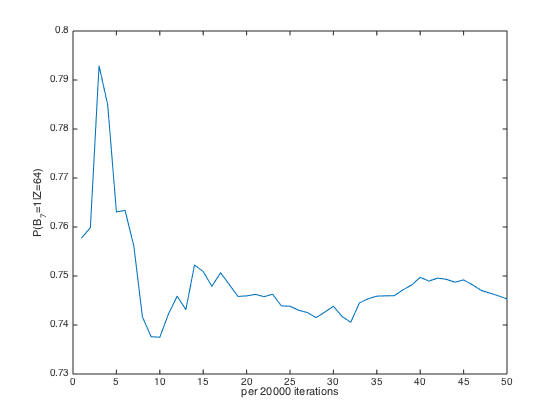
\includegraphics[width=8cm]{3.2c.png}
	\caption{$P (B_7 = 1|Z = 64)$ as a function of the number of samples}
	\label{3.2c}
\end{figure}

\subsection*{3.3 Node clustering}
CPTs for the polytree is shown in Tab. \ref{3.3}.
\begin{table}[h]
	\centering
	\begin{tabular}{|c|c|c|c|c|c|c|c|}
		\hline
		$Y_1$ & $Y_2$ & $Y_3$ & $Y$ & $P(Y|X=0)$ & $P(Y|X=1)$ & $P(Z_1=1|Y)$ & $P(Z_2=1|Y)$ \\
		\hline
		0 & 0 & 0 & 1 & 0.09375 & 0.09375 & 0.9 & 0.1\\
		\hline
		1 & 0 & 0 & 2 & 0.28125 & 0.09375 & 0.8 & 0.2\\
		\hline
		0 & 1 & 0 & 3 & 0.09375 & 0.03125 & 0.7 & 0.3\\
		\hline
		0 & 0 & 1 & 4 & 0.03125 & 0.28125 & 0.6 & 0.4\\
		\hline
		1 & 1 & 0 & 5 & 0.28125 & 0.03125 & 0.5 & 0.5\\
		\hline
		1 & 0 & 1 & 6 & 0.09375 & 0.28125 & 0.4 & 0.6\\
		\hline
		0 & 1 & 1 & 7 & 0.03125 & 0.09375 & 0.3 & 0.7\\
		\hline
		1 & 1 & 1 & 8 & 0.09375 & 0.09375 & 0.2 & 0.8\\
		\hline
	\end{tabular}
	\caption{CPTs for the polytree}
	\label{3.3}
\end{table}

\subsection*{3.4 Maximum likelihood estimation}
\subparagraph*{(a)}
\begin{equation*}
P(X_{t+1}=x'|X_t=x) = \frac{COUNT_t(x,x')}{COUNT_t(x)}~~1 \le t < T
\end{equation*}

\subparagraph*{(b)}
\begin{equation*}
P(X_{t}=x|X_{t+1}=x') = \frac{COUNT_t(x,x')}{COUNT_{t+1}(x')}~~1 \le t < T
\end{equation*}

\subparagraph*{(c)}
We first derive joint distribution from G1:
\begin{eqnarray*}
P(X_1 = x_1, X_2 = x_2, ... , X_T = x_T) &=& P(X_1 = x_1)\prod_{i=2}^{T}P(X_i = x_i|X_1 = x_1,...,X_{i-1} = x_{i-1})~~(product rule)\\
&=& P(X_1 = x_1)\prod_{i=2}^{T}P(X_i = x_i|X_{i-1} = x_{i-1})~~(d-separation \RNum{1})\\
&=& \frac{COUNT_1(x_1)}{|data|} \prod_{i=1}^{T-1}\frac{COUNT_i(x_i,x_{i+1})}{COUNT_i(x_i)}\\
&=& \frac{\prod_{i=1}^{T-1}COUNT_i(x_i,x_{i+1})}{|data|\prod_{i=2}^{T-1}COUNT_i(x_i)}
\end{eqnarray*}

where $|data|$ is the size of the data set. Then we derive joint distribution from G2:
\begin{eqnarray*}
	P(X_1 = x_1, X_2 = x_2, ... , X_T = x_T) &=& P(X_T = x_T)\prod_{i=1}^{T-1}P(X_i = x_i|X_{i+1} = x_{i+1},...,X_{T} = x_{T})~~(product rule)\\
	&=& P(X_T = x_T)\prod_{i=1}^{T-1}P(X_i = x_i|X_{i+1} = x_{i+1})~~(d-separation \RNum{1})\\
	&=& \frac{COUNT_T(x_T)}{|data|} \prod_{i=1}^{T-1}\frac{COUNT_i(x_i,x_{i+1})}{COUNT_{i+1}(x_{i+1})}\\
	&=& \frac{\prod_{i=1}^{T-1}COUNT_i(x_i,x_{i+1})}{|data|\prod_{i=2}^{T-1}COUNT_i(x_i)}
\end{eqnarray*}

We find the derived joint distribution from G1 and G2 is the same.

\subsection*{3.5 Statistical language modeling}
\subparagraph*{(a)}
The results are displayed in Tab. \ref{3.5a}.
\begin{table}
	\centering
	\begin{tabular}{|p{4cm}|p{4cm}|}
		\hline
		Token & $P_u(w)$ \\
		\hline
		MILLION & 0.002073 \\
		\hline
		MORE & 0.001709 \\
		\hline
		MR. & 0.001442 \\
		\hline
		MOST & 0.000788 \\
		\hline
		MARKET & 0.000780 \\
		\hline
		MAY & 0.000730 \\
		\hline
		M. & 0.000703 \\
		\hline
		MANY & 0.000697 \\
		\hline
		MADE & 0.000560 \\
		\hline
		MUCH & 0.000515 \\
		\hline
		MAKE & 0.000514 \\
		\hline
		MONTH & 0.000445 \\
		\hline
		MONEY & 0.000437 \\
		\hline
		MONTHS & 0.000406 \\
		\hline
		MY & 0.000400 \\
		\hline
		MONDAY & 0.000382 \\
		\hline
		MAJOR & 0.000371 \\
		\hline
		MILITARY & 0.000352 \\
		\hline
		MEMBERS & 0.000336 \\
		\hline
		MIGHT & 0.000274 \\
		\hline
		MEETING & 0.000266 \\
		\hline
		MUST & 0.000267 \\
		\hline
		ME & 0.000264 \\
		\hline
		MARCH & 0.000260 \\
		\hline
		MAN & 0.000253 \\
		\hline
		MS. & 0.000239 \\
		\hline
		MINISTER & 0.000240 \\
		\hline
		MAKING & 0.000212 \\
		\hline
		MOVE & 0.000210 \\
		\hline
		MILES & 0.000206 \\
		\hline
	\end{tabular}
	\caption{Tokens that start with the letter “M” and their numerical unigram probabilities}
	\label{3.5a}
\end{table}

\subparagraph*{(b)}
The ten most likely words to follow the word “THE”, along with their numerical bigram probabilities, are shown in Tab. \ref{3.5b}.

\begin{table}[h]
	\centering
	\begin{tabular}{|p{5cm}|p{5cm}|}
		\hline
		Token & $P_b(w|\mathbf{THE})$ \\
		\hline
		\textlangle UNK \textrangle & 0.615020 \\
		\hline
		U. & 0.013372 \\
		\hline
		FIRST & 0.011720 \\
		\hline
		COMPANY & 0.011659 \\
		\hline
		NEW & 0.009451 \\
		\hline
		UNITED & 0.008672 \\
		\hline
		GOVERNMENT & 0.006803 \\
		\hline
		NINETEEN & 0.006651 \\
		\hline
		SAME & 0.006287 \\
		\hline
		TWO & 0.006161 \\
		\hline
	\end{tabular}
	\caption{10 most probable token after \textbf{THE}}
	\label{3.5b}
\end{table}

\subparagraph*{(c)}
\begin{eqnarray*}
\mathcal{L}_u &=& \log[P_u(\mathbf{the}) P_u(\mathbf{stock}) P_u(\mathbf{market}) ... P_u(\mathbf{points}) P_u(\mathbf{last}) P_u(\mathbf{week})]\\
&=&-64.5094403436\\
\mathcal{L}_b &=& \log[P_b(\mathbf{the|\langle s \rangle}) P_b(\mathbf{stock|the}) P_b(\mathbf{market|stock}) ... P_b(\mathbf{last|points}) P_b(\mathbf{week|last})]\\
&=&-40.9181321338\\
\end{eqnarray*}

Bigram model yields the highest log-likelihood.

\subparagraph*{(d)}
\begin{eqnarray*}
	\mathcal{L}_u &=& \log[P_u(\mathbf{the}) P_u(\mathbf{sixteen}) P_u(\mathbf{officials}) ... P_u(\mathbf{sold}) P_u(\mathbf{fire}) P_u(\mathbf{insurance})]\\
	&=&-44.2919344731\\
	\mathcal{L}_b &=& \log[P_b(\mathbf{the|<s>}) P_b(\mathbf{sixteen|the}) P_b(\mathbf{officials|sixteen}) ... P_b(\mathbf{fire|sold}) P_b(\mathbf{insurance|fire})]\\
	&=&\log(0.0)\\
\end{eqnarray*}

When the pairs (\textbf{sisteen, officials}) and (\textbf{sold, fire}) are not observed in the training corpus? This makes the estimated probability to $\log(0)$, which is meaningless.

\subparagraph*{(e)}

Fig. \ref{3.5e} shows the value of this log-likelihood $\mathcal{L}_m$ as a function of the parameter $\lambda \in [0,1]$. And the optimal $\lambda$ is 
0.65 with probability -42.9642.
\begin{figure}[h]
	\centering
	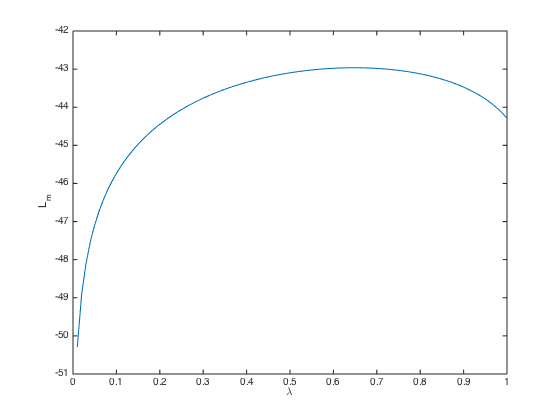
\includegraphics[width=8cm]{3.5e.png}
	\caption{log-likelihood function $\mathcal{L}_m$}
	\label{3.5e}
\end{figure}
\end{document}

